\documentclass[a4paper]{article}
\usepackage[spanish]{babel}
\title{Trabajo Práctico 3}

\usepackage[utf8]{inputenc}
\usepackage{caratula}
\usepackage{graphicx}
\usepackage{color}
\usepackage{listings}
\usepackage{float}
\usepackage{amsmath}
\usepackage{amsfonts}
\usepackage{amssymb}
\usepackage{verbatim}
%%\usepackage{mathtools}


\setlength{\leftmargin}{2cm}
\setlength{\rightmargin}{2cm}
\setlength{\oddsidemargin}{-1cm}
\setlength{\evensidemargin}{-1cm}
\setlength{\topmargin}{-1cm}
\setlength{\textwidth}{18cm}
\setlength{\textheight}{25cm}

\usepackage{fancyhdr}
\pagestyle{fancy}
\fancyhf{}
\fancyhead [LO,LE]{\scriptsize Trabajo Práctico N$^{\circ}$3}
\fancyhead [RO,RE]{\scriptsize Mancuso, Mataloni, Tolchinsky}
\fancyfoot[CE,CO]{\thepage}
\renewcommand{\footrulewidth}{0.4pt}

\usepackage[pdftex, bookmarks=true, colorlinks, citecolor=black, linkcolor=black]{hyperref}
\usepackage{multirow}
\usepackage{multicol}

\begin{document}

\materia{Métodos Numéricos}
\submateria{Primer Cuatrimestre de 2012}
\titulo{Cuando pase el temblor...}
\subtitulo{Autovalores}
\grupo{Trabajo Práctico N$^{\circ}$3}

\integrante{Mancuso, Emiliano}{597/07}{emiliano.mancuso@gmail.com}
\integrante{Mataloni, Alejandro}{706/07}{amataloni@gmail.com}
\integrante{Tolchinsky, Lucas}{591/07}{lucas.tolchinsky@gmail.com}
\resumen{}

\maketitle

\newpage

\addcontentsline{toc}{section}{Índice}
\tableofcontents

% Main document

\newpage

\section{Introducción Teórica}

%Contendr ́a una breve explicaci ́on de la base te ́orica que fundamenta los m ́etodos involu- crados en el trabajo, junto con los m ́etodos mismos. No deben incluirse demostraciones de propiedades ni teoremas, ejemplos innecesarios, ni definiciones elementales (como por ejemplo la de matriz sim ́etrica). En vez de definiciones b ́asicas es conveniente citar ejemplos de bibliograf ́ıa adecuada. Una cita vale m ́as que mil palabras.

En este trabajo práctico debemos calcular las \textit{frecuencias naturales} de un estacionamiento de varios pisos ante un hipotético terremoto, y como distribuir los automóviles para que se encuentre a salvo. Para esto, el trasfondo teórico propuesto por la cátedra toma en cuenta el peso de cada piso y el desplazamiento horizontal de cada uno respecto del suelo. Con estos datos armamos una ecuación por piso logrando un sistema de ecuaciones que en su forma matricial consiste en una \textbf{matriz de tres bandas}. Calculando los \textit{autovalores} de esta matriz es como obtenemos las \textit{frecuencias naturales} necesarias para el desarrollo del problema.

\subsection{Autovalores}
El primer paso en este trabajo consiste en calcular los \textit{autovalores} de una matriz y para lograrlo utilizamos el \textit{Algoritmo QR} que es un método iterativo basado en la \textit{factorización QR} de una matriz. Este algoritmo es en verdad bastante simple; siendo $A = Q_0 \times R_0$ la matriz a la cual queremos calcularle los \textit{autovalores}, formamos la matriz $A_1 = R_0 \times Q_0$ y repetimos lo mismo para calcular $A_2$. En definitiva, el algoritmo genera una serie de matrices de la forma

$$A_{i + 1} = R_i \times Q_i$$

la cual tiende a ser una matriz cuya diagonal principal contiene los \textit{autovalores} de \textit{A}. Cabe destacar que $A_i$ tiende a ser una \textbf{matriz diagonal} si \textit{A} es \textbf{simétrica} o a una \textbf{matriz triangular superior} si no lo es.\\

\subsection{Factorización QR}

Sea $A\in\mathbb{R}^{n\times n}$, la \textit{factorizacion QR} de $A$ es 

$$A = QR$$ 

donde $Q$ una matriz ortogonal y $R$ es una matriz triangular superior.\\

Existen varios métodos para obtener ésta factorizacion: \textit{Householder}, \textit{Givens} y \textit{Gram-Schmidt}.
 

\subsection{Rotaciones de Givens}

El método de \textit{Rotaciones de Givens} es utilizado para obtener la \textit{factorización QR} de una matriz que en nuestro caso es de tres bandas. Por esta razón los únicos valores que hacen falta eliminar son los de la banda por debajo de la diagonal principal de \textit{A}, que llamaremos $b_i$, como mostramos en la \texttt{figura 1}.

\begin{multicols}{2}
\begin{figure}[H]
$$
 \begin{pmatrix}
   a_1 & c_1 & \hdotsfor{4} \\
   b_2 & a_2 &  c_2 & \hdotsfor{3} \\
  \hdots & b_3 & a_3 & c_3 & \hdotsfor{2} \\
   & & \ddots \\
   \hdotsfor{2} & b_i & a_i & c_i & \hdots \\
   & & & & \ddots \\
   \hdotsfor{4} & b_n & a_n \\
 \end{pmatrix}
$$
 \caption{matriz de tres bandas. Los $\cdots$ representan ceros.}
\end{figure}

\begin{figure}[H]
$$
 \begin{pmatrix}
   a_1 & c_1 & c'_1 & \hdotsfor{3} \\
   \hdots & a_2 &  c_2 & c'_2 &\hdotsfor{2} \\
   \hdotsfor{2} & a_3 & c_3 & c'_3 & \hdots \\
   & & \ddots \\
   \hdotsfor{2} & a_{i - 1} & c_{i - 1} & c'_{i - 1} & \hdots \\
   \hdotsfor{3} & a_i & c_i & \hdots \\
   & & & & \ddots \\
   \hdotsfor{4} & b_n & a_n \\
 \end{pmatrix}
$$
 \caption{matriz $R_i$ de Givens. Los $\cdots$ representan ceros.}
\end{figure}
\end{multicols}

En cada iteración de \textit{Givens} el algoritmo transforma la matriz \textit{A} en una \textbf{matriz triangular superior} eliminando $b_i$ y agregando $c'_i$ por encima de la banda superior (\texttt{figura 2}). Para esto en cada iteración se arma una \textit{matriz $P_i$ de rotación} (que es igual a la identidad salvo por cuatro valores) y se la la multiplica por izquierda con $R_i$. La matriz \textit{Q} se obtiene multiplicando las \textit{matrices de rotación} anteriores.\\



\section{Desarrollo}


En este trabajo debiamos calcular las \textit{frecuencias naturales} de un edificio para asegurar que se encuentra seguro frente a un posible terremoto. Para esto calculamos la matriz $A = M^{-1}K$ asociada, siendo $M$ la matriz diagonal con las masas de los pisos y $K$ una matriz tridiagonal con los coeficientes adecuados. Siendo $\lambda_i < 0$ con $i = 1 \hdots n$ los autovalores de $A$, las \textit{frecuencias naturales} están dadas por $\sqrt{-\lambda_i}$. Por lo tanto nuestro trabajo se reducia a ir modificando el edificio (moviendo los autos de lugar) y aplicar un método numérico para calcular los \textit{autovalores} de la matriz $A$ correspondiente a cada configuración del mismo para asegurar que las \textit{frecuencias naturales} no se corresponden con las del terremoto.\\


Para calcularlos utilizamos el \textit{Algoritmo QR}. Sabiendo esto el principal desafío es obtener la \textit{factorización QR} de la matriz para lo cual tuvimos en cuenta dos algoritmos conocidos: \textit{Householder} y \textit{Givens}.
En un principio consideramos utilizar el algoritmo de \textit{Householder} pues en una primera impresión parecía ser más sencillo de mantener, dado que en su iteración iésima pone en cero todos los valores debajo de la diagonal de la iésima columna, no es necesario preocuparse granularmente por cada operación que cancela un valor.\\
Sin embargo en un análisis posterior nos dimos cuenta que siendo que la matriz a factorizar es de tres bandas, el algoritmo de \textit{Givens} sólo necesita anular los valores de la banda que se encuentra por debajo de la diagonal y dado que en la clase teórica estudiamos que este algoritmo se comporta mejor con matrices ralas, consideramos que implementar \textit{Givens} era el acercamiento más apropiado para el problema.\\

A la hora de implementar el algoritmo decidimos optimizar el espacio y no guardar los ceros que contiene nuestra matriz, con lo cual la primer representación consistió de tres un \texttt{arrays}, uno por cada banda. Y dado que la banda inferior se convierte en ceros y aparece una nueva banda por encima de la $c_i$ no necesitamos de más estructura que esta para guardar los datos. El problema con esta propuesta fue que las multiplicaciones eran complicadas de programar y que no podíamos representar otro tipo de matriz. Descartamos esta estructura rápidamente y terminamos implementando las matrices como \texttt{arrays de doubles} aunque tuviéramos que guardar los ceros extra, además, dado que la matriz tiene una fila por cada piso y los edificios de estacionamiento difícilmente sean muy altos, el espacio desperdiciado no es tan significativo.

\subsection{Algoritmo QR: criterios de parada}

El \textit{Algoritmo QR} es un algoritmo iterativo es decir que en cada iteración del procedimiento se mejora el resultado, pero cuándo terminar de iterar es algo que no está definido y depende de la situación. En nuestro caso sabemos que la matriz resultante tiende a ser \textbf{diagonal} o \textbf{triangular superior} y de cualquier manera la \textbf{triangular inferior} tiende a cero. Teniendo en cuenta esto, el criterio de parada que elegimos consiste en realizar la \textbf{suma del módulo} de los elementos de la \textbf{triangular inferior} y comparar este valor con la suma de la iteración anterior, si dicha suma es menor a un $\epsilon > 0$ (parámetro de nuestro programa), terminamos el algoritmo.\\
Lo cierto es que no hay garantía de que al acercarse la \textbf{triangular inferior} a cero los valores en la diagonal se parezcan a los \textit{autovalores} y es por esto que probar este criterio de parada y asegurarnos buenos resultados va a ser parte de nuestra experimentación.

\subsection{Heurísticas}

Una manera de solucionar el problema es ir revisando todas las posibles distribuciones de autos, e ir verificando si las \textit{frecuencias naturales} son seguras para esa configuración. Siendo \textit{n} el número de pisos, \textit{p} y \textit{m} la cantidad de autos pesados y livianos respectivamente, la cantidad total de configuraciones es $n^l \times n^p$ haciendo que éste procedimiento sea computacionalmente caro. Por lo tanto el enfoque más práctico es realizar algoritmos heurísticos para encontrar una solución y a continuación exponemos las estrategias utilizadas:

\begin{itemize}
  \item \textbf{Random}. Esta es la heurística más sencilla, consiste en dar una distribución aleatoria de los autos en el edificio y verificar si es una solución. Esto se repite hasta encontrar una solución.
  \item \textbf{Mover un auto pesado}. Este algoritmo elige un piso de manera aleatoria y mueve un auto pesado a otro piso, también elegido al azar.
  \item \textbf{Intercambiar dos autos}. Muy similar al algoritmo anterior, solo que en este caso intenta intercambiar un auto pesado por uno liviano en dos de los pisos. De no haber dos autos disponibles para ello, realiza un movimiento.
\end{itemize}

Notemos cómo en las heurísticas propuestas siempre hay un grado de aleatoriedad. Esto se debe a que no existe una relación ponderable entre las \textit{frecuencias naturales} del edificio y la  distribución de los autos o el peso de los pisos. Tan solo mover un auto de un piso a otro puede alterar por completo las frecuencias y por eso creemos que no tiene mucho sentido tomar una decisión arbitraria para elegir qué movimiento realizar. 

\subsection{Heurísticas alternativas}

A la vista de la naturaleza de este problema, donde no es posible determinar una mejora en las \textit{frecuencias naturales} dado un movimiento y decidimos utilizar heurísticas aleatorias, nos encontramos con el problema de que muchas veces no nos es posible obtener una solución, por ejemplo, para el archivo \texttt{prueba20.txt} ninguna de nuestras heurísticas es capaz de dar una configuración que satisfaga el problema. Esto se debe a que las combinaciones que generan nuestros algoritmos son muy diversas y desorganizadas. Por esto decidimos explorar otra alternativa y barrer un conjunto de combinaciones más reducido, con la esperanza de que entre ellas encontremos una solución.

\begin{enumerate}
  \item \textbf{Pesados abajo, livianos arriba}. Este algoritmo lo que hace es, empezando por planta baja y último piso, subir los autos livianos y bajar los pesados. Cuando no puede hacer más intercambios, pasa al primer y el anteúltimo piso, repitiendo este procedimiento para todo el edificio.
  \item \textbf{Distribuir los livianos}. Esta heurística busca distribuir los autos livianos en todos los pisos. Comienza llevando todos a planta baja para luego ir moviendo un auto a cada uno de los demás pisos. Esto se repite hasta quedarse sin autos donde pasa a repartir los que hay en el primer piso. Cuando el algoritmo acumula todos los autos livianos en el último piso, termina. Cabe destacar que luego de mover un auto se prueba si la distribución es una solución.
  \item \textbf{Distribuir los pesados}. Idem el algoritmo anterior, pero para autos pesados.
  \item \textbf{Distribución pesados y livianos}. Para este algoritmo utilizamos los dos anteriores de manera alternada. Primero moviendo un liviano y luego un pesado.
\end{enumerate}

%Deben explicarse los m ́etodos num ́ericos que utilizaron y su aplicaci ́on al problema concreto involucrado en el trabajo pr ́actico. Se deben mencionar los pasos que si- guieron para implementar los algoritmos, las dificultades que fueron encontrando y la descripci ́on de c ́omo las fueron resolviendo. Explicar tambi ́en c ́omo fueron planteadas y realizadas las mediciones experimentales. Los ensayos fallidos, hip ́otesis y conjeturas equivocadas, experimentos y m ́etodos malogrados deben figurar en esta secci ́on, con una breve explicaci ́on de los motivos de estas fallas (en caso de ser conocidas).

\newpage

\section{Resultados y Discusión}

A la hora de poner a prueba nuestro programa, decidimos dividir en análisis en dos partes: el \textit{Algoritmo QR} y las \textit{heurísticas}. Esto se debe a que estas dos etapas del algoritmo son de naturaleza muy distinta, una por su rigor matemático y la otra por el factor  aleatorio que introduce.

\subsection{Algoritmo QR}

\begin{comment}
Por eso lo que hicimos fue buscar una instancia solución al problema de 3, 5 y 10 pisos provisto por la cátedra con una de nuestras heurísticas y utilizar eso como dato de entrada. De esta manera lo único que tiene que realizar el algoritmo es el cálculo de los \textit{autovalores} para verificar que el edificio no sufrirá consecuencias del terremoto.

Las instancias utilizadas para estas pruebas son las siguientes:

\vspace{2em}
\textit{3 pisos de 236.500kg, 150 autos de 500kg y 150 autos de 1000kg}
\begin{center}
\begin{tabular}{|c|c|c|}
  \hline
  Piso & Livianos & Pesados \\
  \hline
1   & 149 & 1     \\
2   & 1     & 144 \\
3   & 0     & 5     \\
\hline
\end{tabular}
\end{center}

\vspace{2em}
\textit{5 pisos de 66.500kg, 200 autos de 500kg y 200 autos de 1000kg}
\begin{center}
\begin{tabular}{|c|c|c|}
  \hline
  Piso & Livianos & Pesados \\
  \hline
1   & 79   & 13   \\
2   & 121 & 0     \\
3   & 0     & 186 \\
4   & 0     & 1     \\
5   & 0     & 0     \\
\hline
\end{tabular}
\end{center}

\vspace{2em}
\textit{10 pisos de 20.000kg, 56 autos de 550kg y 56 autos de 900kg}
\begin{center}
\begin{tabular}{|c|c|c|}
  \hline
  Piso & Livianos & Pesados \\
  \hline
1   & 1   & 6   \\
2   & 19 & 0   \\
3   & 0   & 0   \\
4   & 22 & 0   \\
5   & 0   & 24 \\
6   & 0   & 0   \\
7   & 0   & 13 \\
8   & 0   & 13 \\
9   & 14 & 0   \\
10  & 0  & 0   \\
\hline
\end{tabular}
\end{center}

Sabiendo que el \textit{Algoritmo QR} es iterativo, pusimos un tope de cantidad de iteraciones que el algoritmo va a realizar en caso de no alcanzar el criterio de parada y nos propusimos estudiar qué sucede con este valor para matrices de distintos tamaños, ajustando el parámetro del criterio de parada en $\epsilon = 0.00001$. Lo que suponemos es que cuanto más grande es la matriz, más iteraciones requiere para afinar los \textit{autovalores}.\\

En la tabla a continuación presentamos los resultados de esta prueba. Para las tres instancias tomamos nota de cuántas iteraciones requiere como mínimo para cumplir con el criterio de parada que hemos fijado. Además observamos otro fenómeno interesante: para la instancia de tamaño 3, si la ejecutamos con menos de 5 iteraciones el algoritmo no detecta que esta es una solución (y por lo tanto, comienzan a trabajar las heurísticas). 

\vspace{2em}
\begin{center}
\begin{tabular}{|c|c|c|}
  \hline
  Pisos & Cumple criterio & Detecta solución \\
  \hline
3   & 26 & 5  \\
5   & 41 & 1  \\
10 & 278 & 1 \\
\hline
\end{tabular}
\end{center}

En un principio el fenómeno ocurrido para la instancia de tres pisos nos resultó bastante extraño, pues la misma es una solución (y lo comprobamos con sus \textit{frecuencias naturales}). Luego de analizar el algoritmo encontramos cuál era la razón detrás de esto y lo que estaba sucediendo era que con una cantidad de iteraciones tan baja, la matriz resultante del \textit{Algoritmo QR} no produce \textit{autovalores} de una calidad suficiente como para que el cálculo de \textit{frecuencias naturales} quede en el rango correspondiente de una solución. Notablemente esto no sucede para instancias más grandes del problema, donde si bien el criterio de parada no se cumple, la primer matriz resultante $A_1 = R_0 \times Q_0$ tiene en su diagonal valores suficientemente cercanos a los \textit{autovalores} como para detectar la solución.\\


En cuanto a la cantidad de iteraciones necesarias para cumplir con el criterio de parada, vemos que la misma aumenta a medida que la matriz asociada crece, y esto tiene bastante sentido dado que son más los valores que deben tender a cero en la \textbf{triangular inferior}.\\

Como próxima evaluación quisimos poner a prueba la tolerancia del criterio de parada elegido y ver cuántas iteraciones le toma al algoritmo desacelerar la convergencia de la \textbf{triangular inferior}. Para esto, utilizamos las mismas instancias que para la prueba anterior y 1000 como cantidad de iteraciones máxima.\\
\end{comment}

En esta primer etapa de la evaluación queremos probar el desempeño del algoritmo que calcula los \textit{autovalores} de la matriz asociada al problema, verificando la calidad de los mismos utilizando diferentes valores de $\epsilon$ para el criterio de parada y comparándolos con los valores obtenidos del programa \textit{Matlab}. Para esto, utilizamos la matriz $A$ correspondiente a un edificio random generado por nosotros \textit{archivosPrueba/random10.txt}. 



\begin{figure}[H]
  \centering
  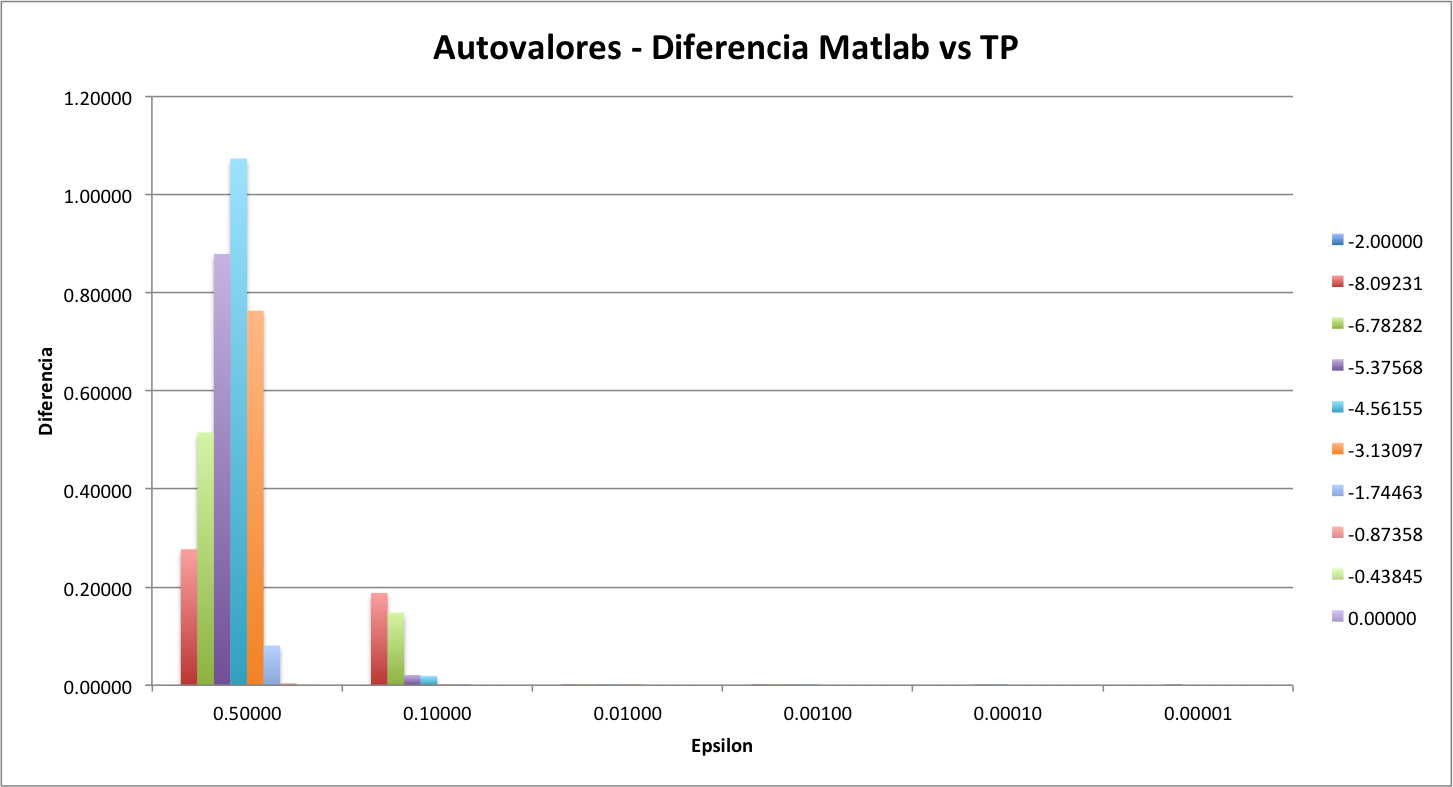
\includegraphics[scale=0.75]{graficos/3-Autovalores.png}
  \caption{Agrupados por $\epsilon$ se muestran los errores que cometemos para los distintos autovalores.}
\end{figure}

Lamentablemente en la \texttt{Figura 3} la diferencia de los autovalores a medida que achicamos el $\epsilon$ es tan chica que no se puede apreciar de forma visual por un tema de escala. Sin embargo, la tabla donde están las diferencias no vale la pena presentarla pues realmente las diferencias son muy pequeñas. Lo importante de esta figura es la notable diferencia que hay para valores de $\epsilon$ más grandes.

Para este trabajo práctico, consideramos que un $\epsilon$ del orden de $10^{-4}$ es aceptable para seguir adelante con la experimentación.


\begin{figure}[H]
  \centering
  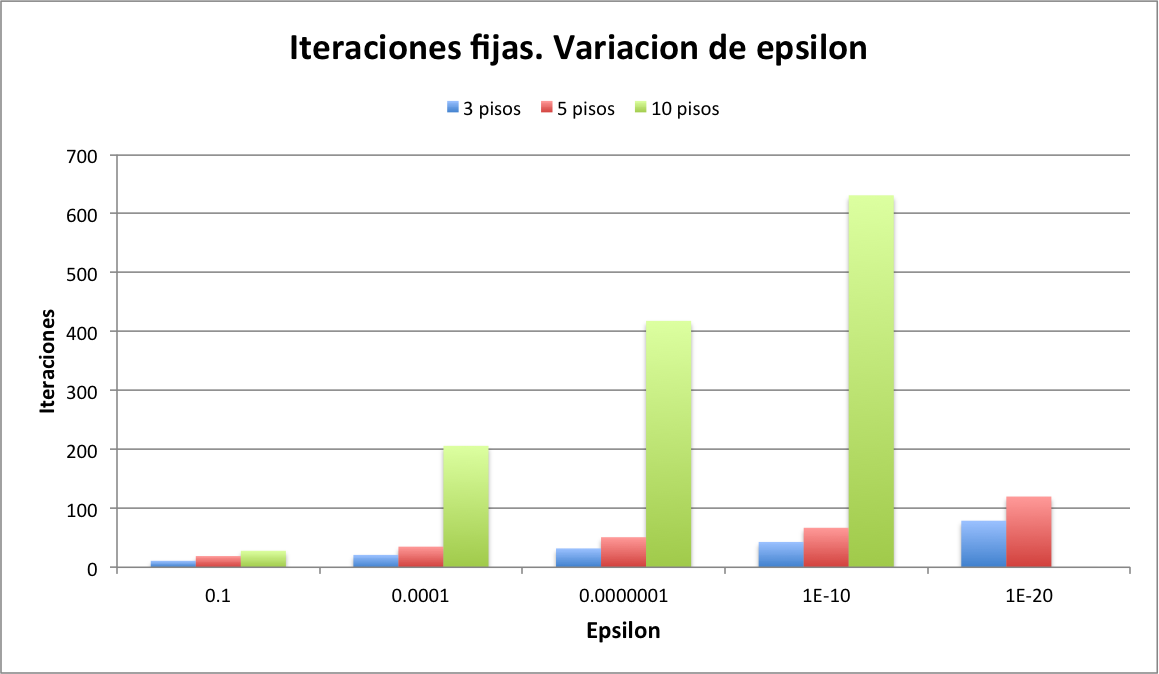
\includegraphics[scale=0.75]{graficos/1-Cantidad_iteraciones_por_piso.png}
  \caption{Agrupados por $\epsilon$ se muestran los distintos edificios y las iteraciones necesarias hasta detenerse. En el ultimo caso, el edificio de 10 pisos corta por iteraciones.}
\end{figure}

La primera impresión que tuvimos al ver los resultados fue la gran diferencia en cantidad de iteraciones entre la instancia de tamaño 10 y la de tamaño 5, siendo que la segunda no está muy lejos de la instancia de tres pisos. De todas maneras podemos ver que lograr una precisión de $1\times 10^{-10}$ en menos de mil iteraciones para es bastante satisfactorio, en especial si tenemos en cuenta que los elementos de la diagonal empiezan a parecerse a los \textit{autovalores} en iteraciones muy tempranas para $\epsilon = 0.00001$.

\subsection{Heurísticas}

%Deben incluir los resultados de los experimentos, utilizando el formato m ́as adecuado para su presentaci ́on. Deber ́an especificar claramente a qu ́e experiencia corresponde cada resultado. No se incluir ́an aqu ́ı corridas de m ́aquina. Algo fundamental en su aprendizaje en la materia es la presentaci ́on de resultados de forma clara y concisa para el lector.

%Se incluira aquı un analisis de los resultados obtenidos en la seccion anterior (se analizara su validez, coherencia, etc.). Deben analizarse como mınimo los ıtems pedidos en el enunciado. No es aceptable decir que “los resultados fueron los esperados”, sin hacer clara referencia a la teor ́ıa a la cual se ajustan. Adem ́as, se deben mencionar los resul- tados interesantes y los casos “patol ́ogicos” encontrados.

\newpage

\section{Conclusiones}
%Esta secci ́on debe contener las conclusiones generales del trabajo. Se deben mencionar las relaciones de la discusi ́on sobre las que se tiene certeza, junto con comentarios y observaciones generales aplicables a todo el proceso. Mencionar tambi ́en posibles extensiones a los m ́etodos, experimentos que hayan quedado pendientes, etc.

\newpage

\section{Apéndices}
\subsection{A - Enunciado}

El trabajo pr\'actico consiste en evaluar la resistencia s\'\i smica de un
edificio de varios pisos que funciona como estacionamiento, proponiendo un plan de
reubicaci\'on de los veh\'iculos lo m\'as eficiente posible.\\

\textbf{El modelo}\\
Consideremos un edificio de $n$ pisos como el de la Figura~1. Un modelo sencillo
para estudiar el efecto de un terremoto sobre el edificio consiste en
considerar cada piso $i=1,\dots,n$ como un bloque de masa $m_i$, unido a los
pisos adyacentes por medio de un conector el\'astico cuya acci\'on se parece
a la de un resorte. Para $i=0,\dots,n-1$, la uni\'on entre los pisos $i$ e
$i+1$ suministra una fuerza de restituci\'on
\begin{displaymath}
F_i\ =\ k_i (x_{i+1}-x_i),
\end{displaymath}
donde $x_i(t)\colon \mathbb{R}_+ \rightarrow \mathbb{R}$ representa el desplazamiento
horizontal del $i$-\'esimo piso en cada instante con respecto al suelo (asumimos que $i=0$ corresponde
al suelo y que $x_0=0$), y los $k_i\in\mathbb{R}_+$ representan los coeficientes
de rigidez. Aplicando la segunda ley de Newton del movimiento %$F = ma$ 
a cada secci\'on del edificio ($m_i\, a_i = F_i-F_{i-1}$, con $a_i$ la aceleraci\'on, que escribiremos como la derivada segunda de $x_i$), 
obtenemos el siguiente sistema de ecuaciones diferenciales ordinarias:
\begin{eqnarray*}
m_1 \ddot{x}_1 & = & -k_0 x_1 + k_1 (x_2-x_1) \nonumber \\
m_2 \ddot{x}_2 & = & -k_1 (x_2-x_1) + k_2 (x_3-x_2) \nonumber \\
m_3 \ddot{x}_3 & = & -k_2 (x_3-x_2) + k_3 (x_4-x_3) \nonumber \\
\vdots &  & \vdots \nonumber \\
m_n \ddot{x}_n & = & -k_{n-1} (x_n-x_{n-1}) \nonumber \\
\end{eqnarray*}
Escrito en forma matricial, este
sistema toma la forma $M\ddot{\mathbf{x}} = K\mathbf{x}$, 
donde $M\in\mathbb{R}^{n\times n}$ es una matriz
diagonal con las masas de los pisos y $K\in\mathbb{R}^{n\times n}$ es una matriz
tridiagonal con los coeficientes de rigidez adecuados. Como $m_i>0$ para
$i=1,\dots,n$, entonces $M$ tiene inversa y el sistema se puede reescribir
como $\ddot{\mathbf{x}} = (M^{-1} K) \mathbf{x} = A\mathbf{x}$, donde $A = M^{-1} K$ tiene autovalores negativos.

Sean $\lambda_1,\dots,\lambda_n$ los autovalores de $A$. Los valores
$\omega_i=\sqrt{-\lambda_i}$, para $i=1,\dots,n$, representan las frecuencias
naturales del sistema, e indican la estabilidad del edificio durante un
terremoto. Si la frecuencia del sismo es muy pr\'oxima a alguna de estas
frecuencias, hay riesgo de que el edificio entre en resonancia y colapse.\\

\textbf{El problema}

Nos encontramos en el 
estacionamiento de una importante concesionaria de autom\' oviles de una reconocida marca,
% dep\'osito de lavarropas de una conocida casa de electrodom\'esticos, 
y se avecina un terremoto sobre nuestra ciudad. 
Contamos con informaci\'on fidedigna provista por nuestro
informante en el Departamento de Geolog\'\i a de la FCEyN 
de que la frecuencia del terremoto ser\'a $\omega = 3\ \hbox{Hz}
= 3 \frac{1}{\hbox{seg}}$.

Para realizar c\'alculos simplificados podemos asumir que todos los autos 
se pueden agrupar en 2 categor\'ias: livianos, de masa $m_l$, y pesados, 
de masa $m_p > m_l$.
Adem\'as, $m_0$ es la masa propia del edificio correspondiente a cada piso.
De esta forma, si el piso $i$ tiene $l_i$ veh\'\i culos livianos y 
$p_i$ veh\'\i culos pesados, entonces su masa es $m_i = m_0 + l_i m_l + p_i m_p$. 
El problema que debemos resolver -y r\'apidamente- consiste en determinar
cu\'antos autos livianos y pesados debemos quitar de cada piso 
(reubic\'andolos en otros pisos) para que ninguna de las frecuencias 
naturales del edificio se encuentre a menos del 10\% de la frecuencia 
$\omega$ del terremoto.
La soluci\'on \'optima del problema es aquella que permite evitar que el
edificio colapse, reubicando la menor cantidad posible de autom\'oviles.\\

\textbf{El enunciado}

El trabajo pr\'actico consiste en implementar un programa que permita 
resolver este problema. La soluci\'on propuesta debe indicar cu\'antos 
autos livianos y cu\'antos pesados quitar de cada piso, y a qu\'e pisos 
se deben llevarlos. 

Deben proponerse (por lo menos) dos m\'etodos (es v\'alido que sean 
heur\'\i sticos) para obtener el plan de reubicaci\'on. El informe 
deber\'a contener los resultados de los experimentos realizados para
compararlos y evaluar cu\'al es mejor. 

El programa debe incluir una implementaci\'on de
alg\'un algoritmo para calcular los autovalores de una matriz cuadrada, que
deber\'a ser utilizado durante el proceso de decisi\'on. Sugerimos implementar
el algoritmo QR para el c\'alculo de autovalores. El programa debe tomar los
datos desde un archivo de texto con el siguiente formato:
\begin{eqnarray}
 & & n\ m_0\ m_l\ m_p \nonumber \\
 & & k_0\ k_1\ \dots\ k_{n-1} \nonumber \\
 & & l_1\ l_2\ \dots\ l_n \nonumber \\
 & & p_1\ p_2\ \dots\ p_n \nonumber
\end{eqnarray}
Se debe retornar la soluci\'on propuesta con este mismo formato.

El programa que obtenga la mejor redistribuci\'on de autom\'oviles se har\'a
acreedor a la medalla \emph{M\'etodos Num\'ericos 2012} al Mejor Redistribuidor Vehicular.\\

\vskip 15pt

\hrule

\vskip 11pt

{\bf \underline{Entrega Final}}

\begin{description}
  \setlength{\itemsep}{0pt}
  \setlength{\parskip}{0pt}
  \setlength{\parsep}{0pt}
 \item[Formato Electr\'onico:] jueves 28 de junio de 2012, hasta las 23:59 hs, a la direcci\'on: 

  {\emph{metnum.lab@gmail.com}}
%  \item[Formato f\'isico y experimentación en clase:] 13 de abril de 2012, de 17 a 21 hs.
 \item[Formato f\'isico:] viernes 29 de junio de 2012, de 17 a 19 hs.
 \item[Competencia entre grupos:] viernes 29 de junio de 2012, 19 hs.
 \item[Entrega de premios:] viernes 29 de junio de 2012, 20:30 hs.
\end{description}


\newpage

%\section{Referencias TODO}
%Es importante incluir referencias a libros, art ́ıculos y p ́aginas de Internet consultados durante el desarrollo del trabajo, haciendo referencia a estos materiales a lo largo del informe. Se deben citar tambi ́en las comunicaciones personales con otros grupos.


\end{document}
